\section{Solution}
\label{sec:solution}

\begin{table*}[!t]
\begin{tabular}{|l|l|l|}
\hline
tweet id & user id & tweet\\
\hline
292375792485298176&858488612& \#KidCudi - \#EraseMe - The Whizz Bells : http://t.co/Lp1zABOV via @youtube\\
292375792481099777&486970282& RT @Kirra\_\_: Today is a day where I need to crawl into my bed and sleep the day away.\\
292375792481099776&336390437& There are poor people, money is the only thing they got.\\
292375792476909568&74570186& I can't do anything without listening to music while I do it.\\
\hline
\end{tabular}
\caption{A sample of the tweet dataset}
\label{tbl:tweets}
\end{table*}


We describe here the PACT program diagram we implemented to produce the statistics on tweets that we want. 
To recap briefly, a PACT program is a generalisation of the Map-Reduce paradigm, in which sequence of second order functions are issued in parallel and combined to execute complex tasks. 
The programming paradigm defines 5 second order functions: map, reduce, match, cross and co-group.
It allows the user to specify any kind of combination between them, in any order.
We propose a flow that uses all the operator except the cross. 
For ease of explanation we describe the PACT program as composed in two different blocks: data cleaning (Section~\ref{sec:cleaning}) and the computation of the statistics (Section~\ref{sec:statistics}).

\subsection{Data cleaning}
\label{sec:cleaning}
In the data cleaning part we take as input a comma separated file having the format $\langle tweet\_id$,$user\_id$,$tweet \rangle$. 
Table~\ref{tbl:tweets} shows an excerpt of the tweet tuples. 
Note that it is not always easy to find interesting information from arbitrarily short-texts.
Therefore, we propose a first flow that tries to remove useless or uninformative tweets by filtering-out the ones that do not contain a minimum portion of english words. 
Figure~\ref{fig:cleaning} depicts the sequence of operations we designed to clean the data in the preliminary phase. 

Once we loaded the tweets into tuples we clean them, from hashtags, user-mentions and urls. 
Tweets are then used in two separate flows: (1) we split them into words in order to count the english words and (2) we perform a sentiment analysis over the text, in order to evaluate the positive and negative polarity expressed by them, as described in Section~\ref{sec:introduction}.
Note that the SentiStrength library is well suited to analyse informal text, so we will apply this evaluation on the whole text, before stemming and further cleaning. 

In order to restrict the search space to those tweets we consider relevant, we import a dictionary of english words and we count english words in each tweet. 
If a tweet has a percentage of english words greater than a threshold $\sigma$ we keep it, otherwise we drop it. 

From the pruned tweets we extract the users, and we assign to the cleaned text the polarities found in the previous step. 

\begin{figure*}[ht]
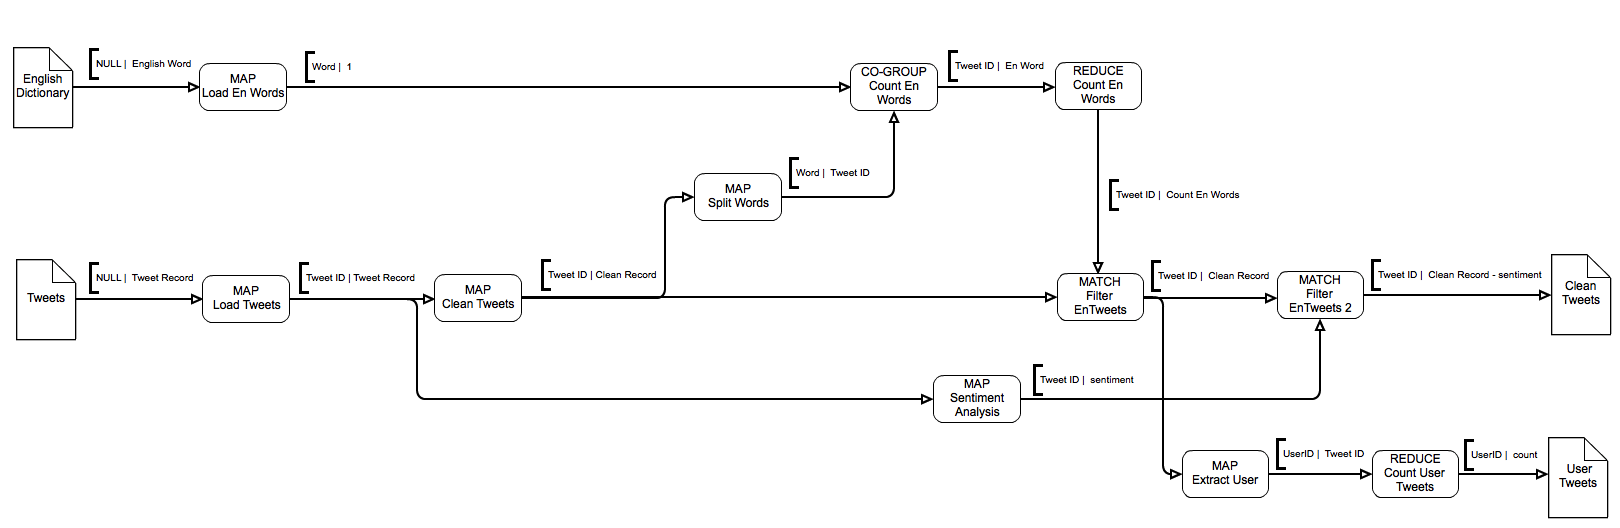
\includegraphics[width=\textwidth]{images/strato_pact_pt1.png} 
\caption{Data cleaning PACT}
\label{fig:cleaning}
\end{figure*}

\subsection{Compute statistics}
\label{sec:statistics}
After having cleaned the raw data and after evaluating text polarities, we compute the statistics using the tuples we have kept in the aforementioned steps. 
First, we load and match the tuples with the tweet timestamp we get from the database.
For each timestamp, we  keep the date and time up to the hour, this means that any further analysis is condensed in a time window of 1 hour.
Second, we match the hashtags with the polarities in order to understand positive and negative trends of the topics. 
It is important to notice that in a tweet more than one hashtag can be present, and we want to analyse each hashtag separately.
This step is performed by a match operation with the sentiment polarities followed by a sequence of reduce operations to compute different statistics.
The first information we want to extract is about the evolution of the popularity of an hashtag.
To obtain this information we will count hour by hour how many tweets contain each hashtag, and similarly we also keep track of how many different users tweet about it.
In the same way we are keeping track, hour by hour, of how popularity changes for each hashtag.
Then we collect for each hashtag the moment in which it reached his peak in popularity alongside the date of first and last appearance, marking in this way the lifespan of the hashtag.



\begin{figure*}[ht]
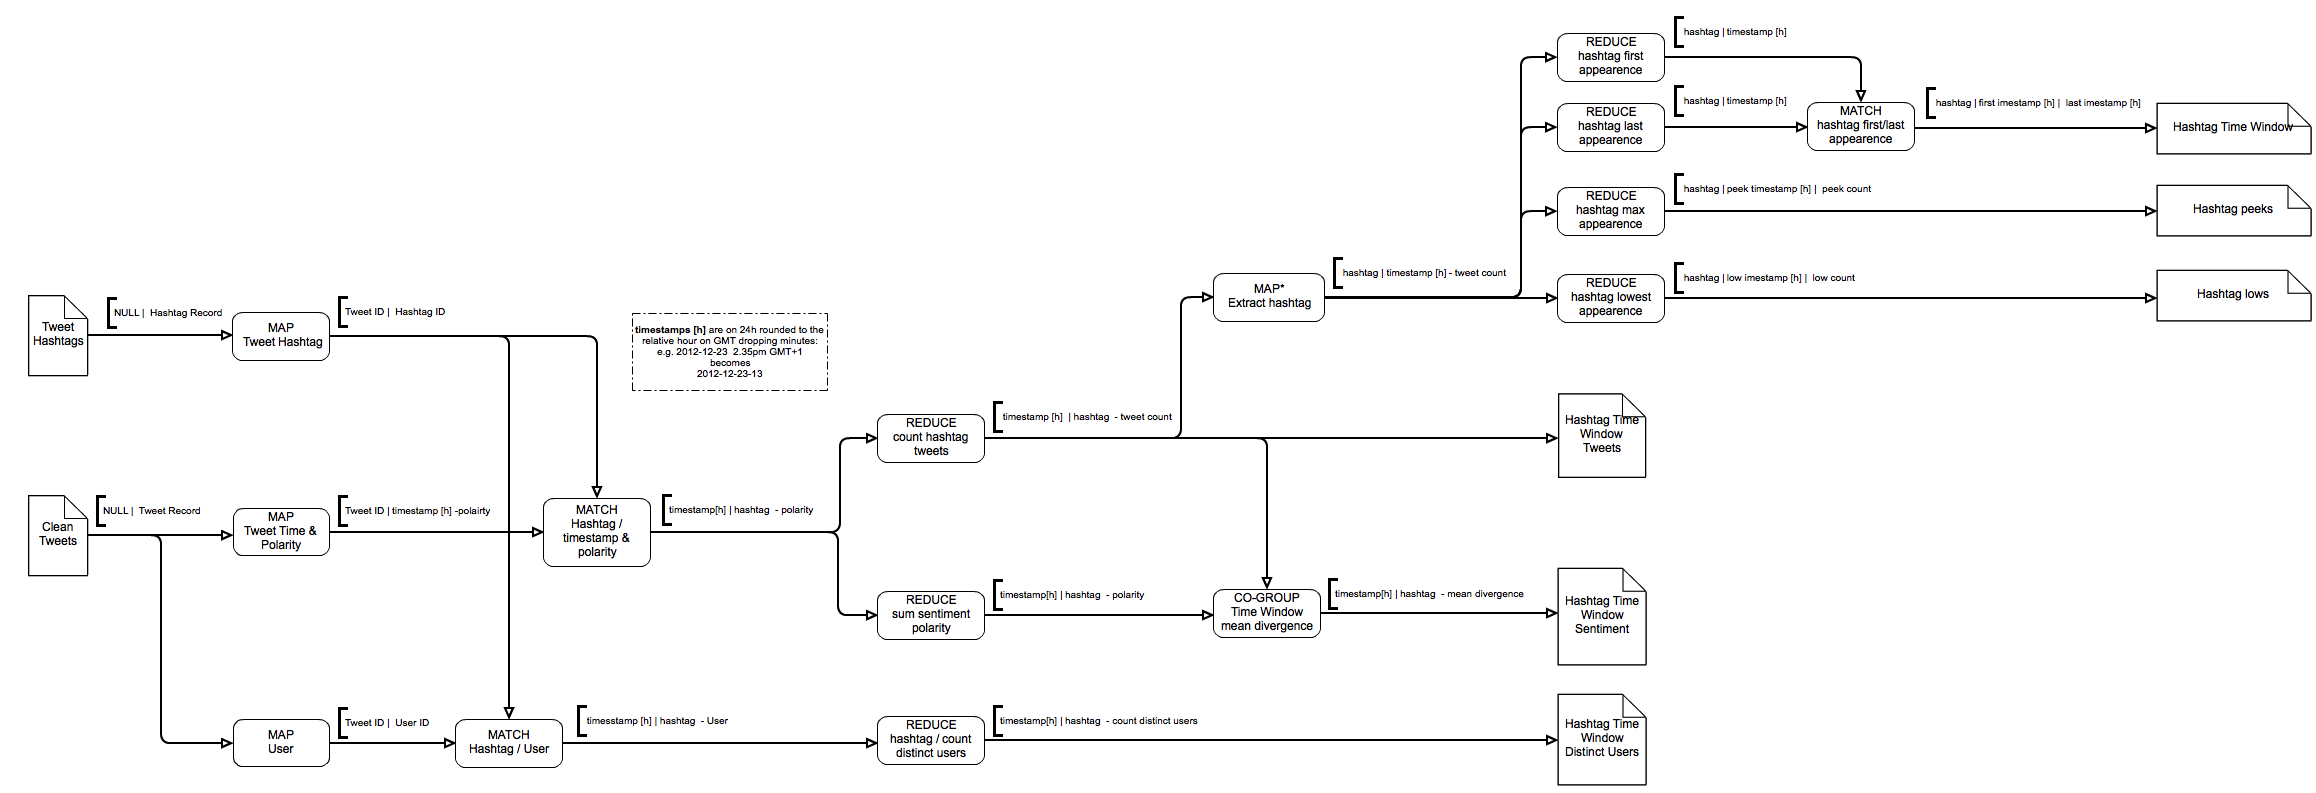
\includegraphics[width=\textwidth]{images/strato_pact_pt2.png} 
\caption{Compute statistics PACT}
\label{fig:statistics}
\end{figure*}
